\section{Description}  
The purpose of the recordings are to obtain several different audio files of music to use for both unit tests and tests on the final system. \\
It is important to know the exact signal on each audio files in order to use it as reference when validating the system. Hence recording of the audio will take place in the anechoic room provided by the acoustic laboratory at AAU. \\
Musical signals and noise is recorded separately. Hereby specific noise can be added to the music digitally in order to gain further control of the signals. \\
Table \ref{tab:audio} makes a list representing the contents of each audio file to be recorded. The contents of the musical audio files is selected on behalf of the complexity of the frequencies - from a single note to a melody played with chords.  \\
Each type of file will be recorded at least two times. This is done to verify the note played and minimize the human mistakes.    \\
The noise to be recorded is chosen to represent additive noise that could appear naturally in a situation where the final system would be used. Note that convolution noise is disregarded as a result of recording in the anechoic room.         
\begin{table}[H]
\centering
\caption{List of recordings in the anechoic room.}
\label{tab:audio}
\begin{tabular}{l|l|l}
\hline
  & \textbf{Music}                      & \textbf{Noise}     \\ \hline
1 & Low E string - long/short           & Random speak       \\ \hline
2 & High E string - long/short          & Curling paper      \\ \hline
3 & Low E chord                         & Random clapping    \\ \hline
4 & High E chord                        & Rhythmical clapping \\ \hline
5 & Melody of single strings - slow/fast & Random cheering    \\ \hline
6 & Melody with chords - slow/fast      & Singing            \\ \hline
\end{tabular}
\end{table}
Beside the listed audio files, which add up to $15$ different files, natural outdoor sound is also recorded outside the anechoic room. 

\subsection{Anechoic room} 
An anechoic room is designed to absorb all reflections from sound or electromagnetic waves. Further the room is isolated from exterior noise, which makes it possible to only record or measure the exact sound that is coming from the instrument without the presence of interfering reflections. \\ The specific room at AAU is build as a box inside a box. The inner box is placed on rubber suspensions, and the inner walls are covered by sound absorbing wedges of about 0.4 m length due to requirements for anechoic performances. The inside dimensions of the room are 4.5 m times 5.0 m with a height of 4.0 m.\cite{anechoic}.\\
Hence, by recording in the anechoic room signal noise is reduced to a minimum.

\section{Procedure}
\textbf{Set up for inside anechoic room:}\\
\begin{itemize}
\item[-] A grid just big enough to support a microphone stand is install as the only floor in the anechoic room, partly covered by wadding. 
\item[-] One man with Guitar sits on the grid, playing into the micophone. 
- microphone is connected to ??? \trine{OBS!} so it connected to the listening/control room besides the anechoic room. 
\end{itemize}   
\textbf{Set up in control room: }
\begin{itemize}
\item[-] Microphone is connected to the ACD, which is connected to the PC.
\item[-] The PC is running the recording program Audacity. From the program the sampling frequency is specified to 44.1 kHz.\trine{tjek samplingsfrekvens}
\item[-] An external sound card are plucked into the PC, to secure optimal sampling.  
\item[-] Though      
\end{itemize}

Table \ref{tab:equip} specifies the equipment used for the recording. Figure \ref{fig:setup1} and \ref{fig:setup2} show the set up inside the anechoic room.   
\begin{table}[H]
\centering
\caption{Equipment list}
\label{tab:equip}
\begin{tabular}{l|l|l}
\hline
  & \textbf{Equipment}                & \textbf{Specifications}                                                                                      \\ \hline
1 & Condenser Microphone, C 414 B-ULS &                                                                                                              \\ \hline
2 & ADC, Roland Quad-capture          & \begin{tabular}[c]{@{}l@{}}Analog $2x2$, digital $2x2$, USB 2.0,\\ 4 in/4 out, 24 bit , 192 kHz\end{tabular} \\ \hline
3 & Soundcard                         &                                                                                                              \\ \hline
4 & PC                                &                                                                                                              \\ \hline
5 & Audacity                          &                                                                                                              \\ \hline
6 & Guitar   	                      &                                                                                                              \\ \hline
7 & Paper   	                      &                                                                                                              \\ \hline
\end{tabular}
\end{table}

\begin{figure}[H]
\centering
	\begin{minipage}{0.49\textwidth}
  	  
    		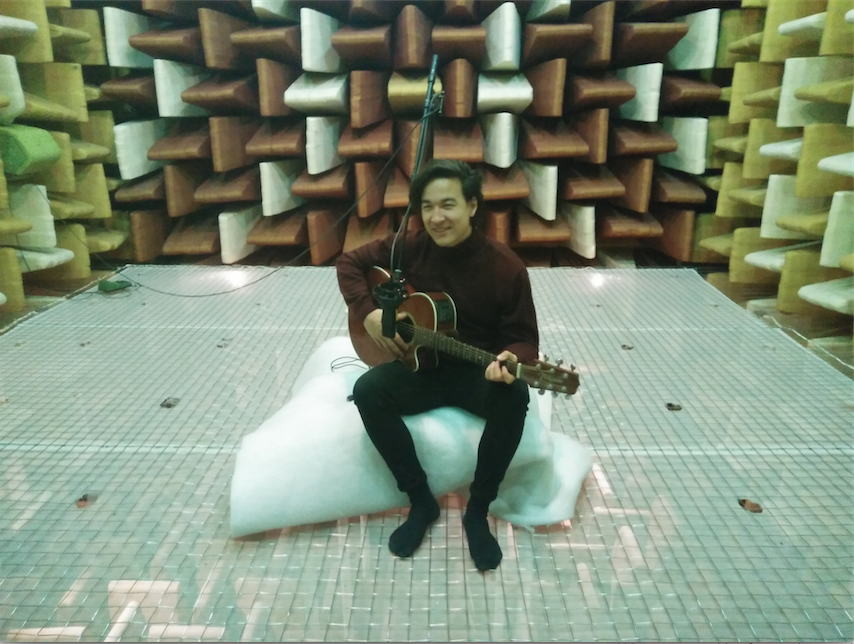
\includegraphics[scale=0.22]{figures/recording/setup1.png}
    		\caption{Set up inside anechoic room.}
    		\label{fig:setup1}
    \end{minipage}
    \begin{minipage}{0.49\textwidth}
  	  
    		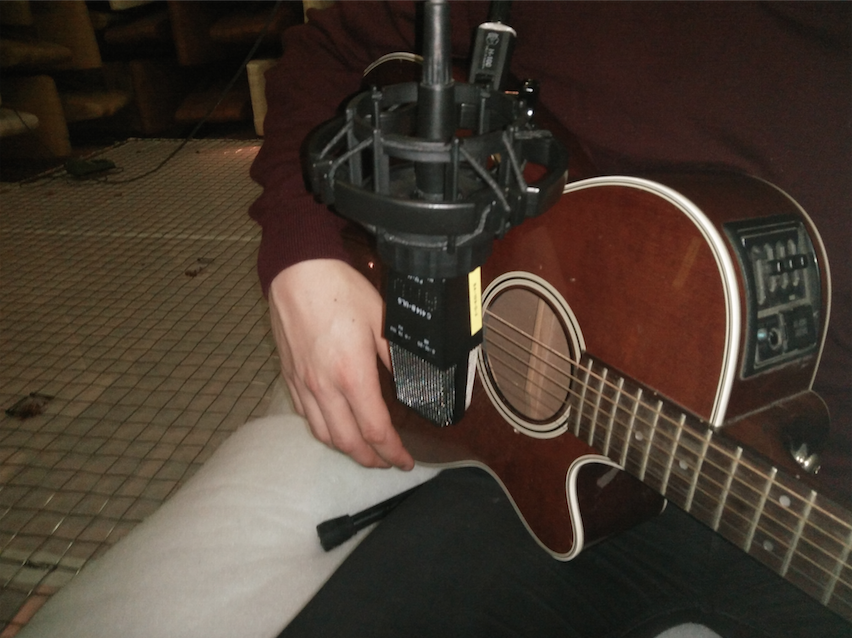
\includegraphics[scale=0.22]{figures/recording/setup2.png}
    		\caption{Set up inside anechoic room.}
    		\label{fig:setup2}
    \end{minipage}
\end{figure} 

\textbf{Recording procedure}\\
Through a communication system the guitar player is told what and when to play by the person controlling Audacity in the control room, who starts and stops the recordings. \\
The procedure for recording the noise follows the same procedure.\\
\\
When recoding the outdoor noise the microphone stand is placed in an open window inside the control room. One long record is taken, which include bird song, car noise, and especially noise from a ventilator. One more more record is made similarly but with low random talking.

\section{Source of errors}
\begin{itemize}
\item[-] Internal noise from microphone will appear. 
\item[-] Minimal reflection of sound signal caused by the floor and the man necessary in the room can occur. 
\item[-] Not playing exactly the note we want to play can make as an error source to consider when validating the final system.
\item[-] The sensibility/gain adjustments to be made on the ADC was adjusted for the recorded sound to not peak within the frequency band provided by Audacity. If a peak is reached without it will cause a an error.            
\end{itemize}

\section{Evaluation}
Usable audio files with minimal amount of noise was obtained from the recording. The noise was minimized by using the anechoic room and further minimizing the amount of equipment and  people in the room.       
A frequency analysis of the recorded signals is described in chapter \ref{ch9}.  

